\section{Bestimmung der Relaxationslänge}

Es wird vorgegangen wie in der Vorbereitung beschrieben. Auf den Abstand $r$ von der Quelle wird eine Unsicherheit von $\Delta r=\SI{1}{\milli\metre}$ angenommen. Die Skalenbreite betrug $\SI{1}{\milli\metre}$, was einer Unsicherheit von $\SI{0,5}{\milli\metre}$ entsprechen würde. Es ist jedoch auch möglich, dass die Quelle ungenau positioniert wurde.
Die Anzahl der detektierten Neutronen folgt einer Poisson-Verteilung, weshalb die Unsicherheit $\Delta N=\sqrt{N}$ beträgt. Da die Fehler unkorreliert sind, wird die gaußsche Fehlerfortpflanzung verwendet. Es ergibt sich für die Unsicherheit von $y=\ln(Nr^{2})$
\begin{equation}
 \Delta y = \sqrt{\frac{1}{N}+\left(\frac{2\Delta r}{r}\right)^{2}}.
\end{equation}

Die lineare Regression der Form $y=ar+b$ wird mit ``kafe'' durchgeführt und ergibt (s. Abb. \ref{fig:plot1})
\begin{equation}
 a = \SI{-0,077\pm0,003}{\per\centi\metre}.
\end{equation}
Daraus folgt für die Relaxationslänge
\begin{equation}
 \lambda = -\frac{1}{a} = \SI{12,9\pm0,5}{\centi\metre}.
\end{equation}

\begin{figure}[tb]
  \centering
  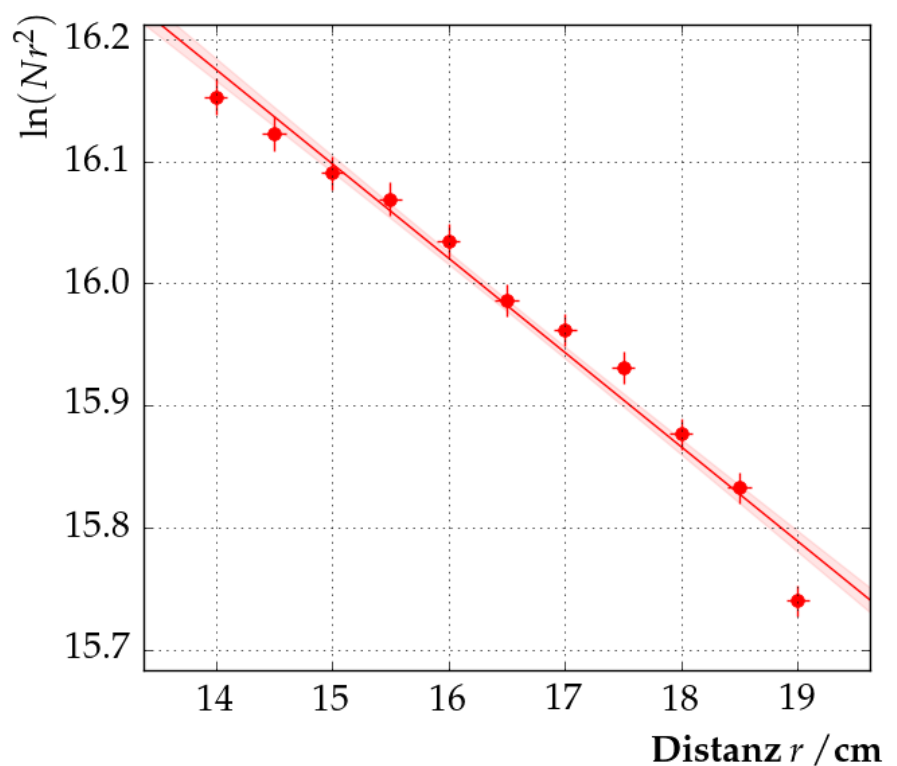
\includegraphics[scale=0.5]{./fig/plot1.png}
  \caption{Lineare Regression zur Bestimmung der Relaxationslänge (ohne Cd-Kugelschale)}
  \label{fig:plot1}
\end{figure}

\begin{figure}[tb]
  \centering
  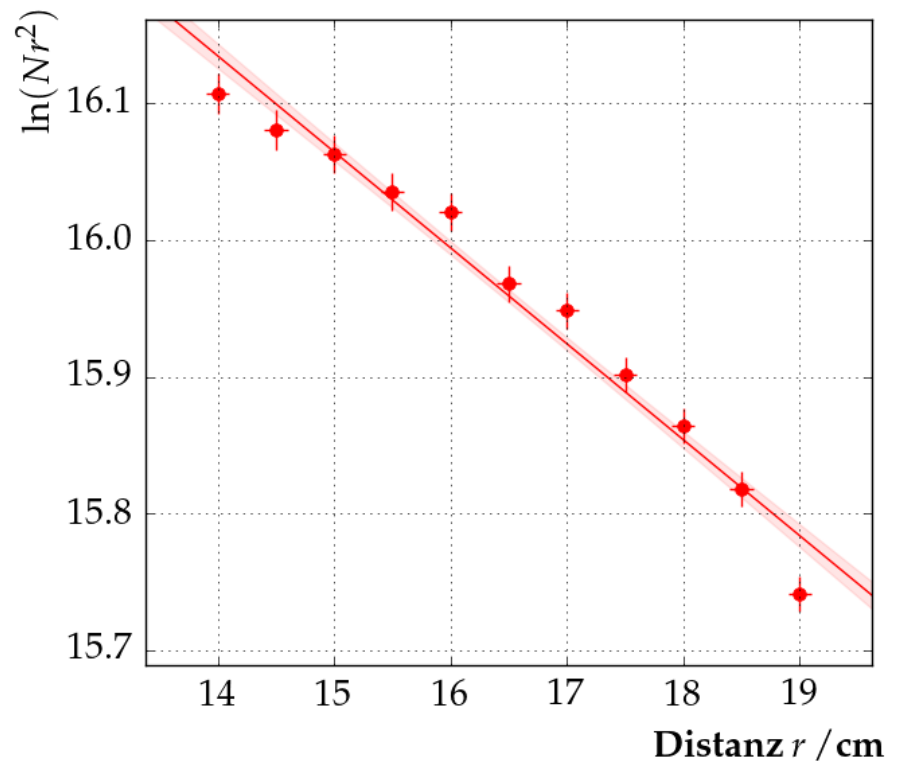
\includegraphics[scale=0.5]{./fig/plot2.png}
  \caption{Lineare Regression zur Bestimmung der Relaxationslänge (mit Cd-Kugelschale)}
  \label{fig:plot2}
\end{figure}

\section{Bestimmung der Diffusionslänge}

\begin{figure}[tb]
  \centering
  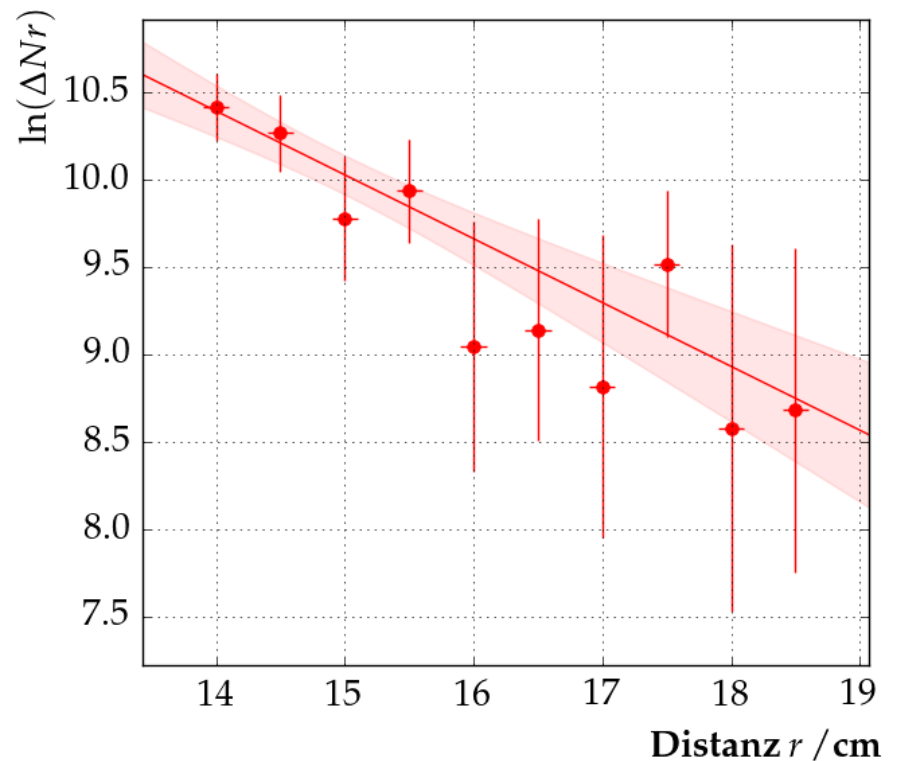
\includegraphics[scale=0.5]{./fig/plot3.png}
  \caption{Lineare Regression zur Bestimmung der Diffusionslänge}
  \label{fig:plot3}
\end{figure}

